\documentclass[12pt, a4paper, openany]{article}
\usepackage[utf8]{inputenc}
\usepackage[T1]{fontenc}

\usepackage{mfirstuc}

% LANGUAGE
\usepackage[english,french]{babel}
    \selectlanguage{french}
    \frenchsetup{StandardItemLabels=true}
\usepackage{enumitem}  % Enumerate improved

% MATH / Others
\usepackage{amsmath, amssymb}  % Math symbols
\usepackage{physics}  % \norm and \abs
\usepackage{esvect, cancel}  % Misc., vectors, strikethrough
\usepackage{mhchem}  % Chemistry
\usepackage{siunitx}  % Units SI
\usepackage{minted}  % Code fences ([cache=false])
\setminted[python]{
    fontsize=\footnotesize,
    tabsize=4,
    rulecolor=black,
    xleftmargin=18pt,
    linenos,
    breaklines
}
\usemintedstyle{pastie}

% GEOMETRY
\usepackage[
    paper=a4paper,
    top=2cm,
    left=2cm,
    headheight=15pt,
    headsep=12pt,
    textwidth=17cm,
    textheight=25.5cm,
]{geometry}
\usepackage{parskip}  % Reformat paragraphs, no indent first line
\usepackage{enumitem}  % Enumerate improved
\usepackage{scrextend}  % Indent text with addmargin environment
\usepackage{graphicx}  % Include graphics
\usepackage{wrapfig}
\graphicspath{{latex-img/}}
\usepackage{caption}  % Caption without figures
\usepackage{float}

\usepackage{paracol}

% HYPERLINKS
\usepackage{hyperref}
\hypersetup{
    colorlinks=true,
    linktoc=all,
    linkcolor=blue,
}

% HEADERS
\usepackage{fancyhdr}
    \pagestyle{fancy}
    \lhead{CS-358 MIT - Project Proposal - Helping Hand}
    \rhead{Lucas Jung (@gruvw)}
    \renewcommand{\footrulewidth}{0.4pt}
    \renewcommand{\headrulewidth}{0.4pt}
\usepackage{etoolbox}  % Define chapter page style
    \patchcmd{\chapter}{\thispagestyle{plain}}{\thispagestyle{fancy}}{}{}

% TITLE PAGE
\title{Helping Hand}
\author{Lucas Jung (IN BA6 324724)\\\url{https://gruvw.com}}
\date{2024 - 03}

\newcommand{\footlink}[2]{\href{#2}{#1}\footnote{{\MakeUppercase #1}: \url{#2}}}
\newcommand*{\fullref}[1]{\hyperref[{#1}]{\autoref*{#1} \nameref*{#1}}}

\begin{document}
\maketitle
\thispagestyle{fancy}
\pagenumbering{arabic}

\begin{center}
    \textbf{Beyond Accessibility: Unleashing the Potential of Home Automation to Foster Independence and Inclusivity for Individuals with Unique Needs}
\end{center}

\vspace{10pt}

\begin{minipage}[t]{0.65\textwidth}
    In the depicted image, you'll find Sean and me.
    Sean, a colleague of my mother, is unfortunately grappling with \href{https://en.wikipedia.org/wiki/ALS}{amyotrophic lateral sclerosis}\footnotemark (ALS), a terminal neurodegenerative disease that progressively diminishes his mobility.
    Presently, he has to spend his days in an electric wheelchair, with only partial movement in his wrists.
    As a result, he relies on others for even the most basic tasks, such as opening a door or operating the lights in his home.
    Despite these challenges, Sean can still manage his smartphone while in his chair, thanks to a specialized joystick and a button.
    The objective of this project is to develop an adaptable solution that empowers people in a similar situation to regain some independence through the use of certain appliances in their home.
\end{minipage}\hfill
\begin{minipage}[t]{0.31\textwidth}
  \centering\raisebox{\dimexpr \topskip-\height}{
  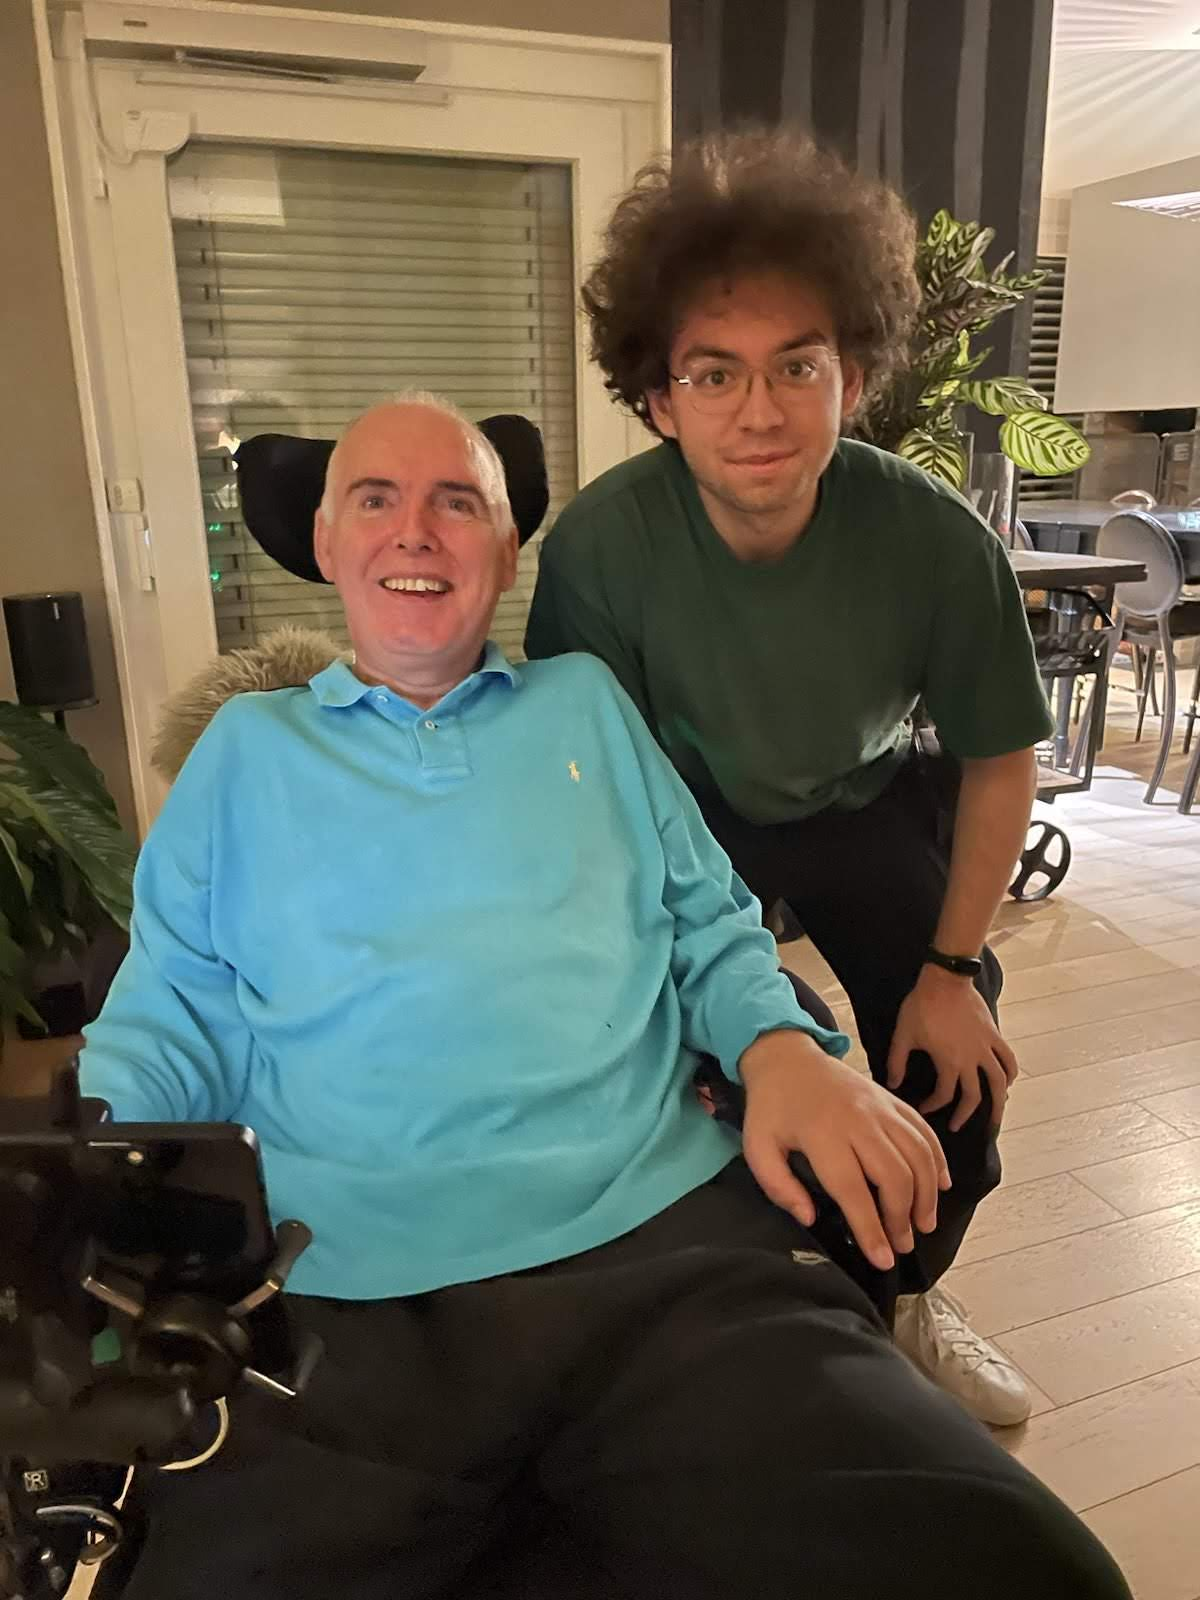
\includegraphics[width=\textwidth]{human.jpg}}
\end{minipage}
\footnotetext{Amyotrophic Lateral Sclerosis: \url{https://en.wikipedia.org/wiki/ALS}}

\vspace{-10pt}

\subsection*{High-level description}

The project aims to create a modular box in which the user can install any one of the various remote controls they have in their home.
The box will be equipped with \footlink{servomotors}{https://en.wikipedia.org/wiki/Servomotor} and a Wi-Fi capable microcontroller, allowing for remote operation of the enclosed remote control by having the motors press on the buttons.
The box must be designed in such a way that the buttons are still usable without causing disruption to a user who prefers direct manual control of the remote.
The design of the case should also be easily adaptable to different type of remote controls.

Each modular box is connected to the Wi-Fi network of the home it is installed in, and the user can command it by using an application on their smartphone.
Naturally, the application will be meticulously designed to maximize \footlink{accessibility}{https://en.wikipedia.org/wiki/Accessibility} for users with limited input capabilities.
Collaborative feedback and discussions with Sean will play a pivotal role in enhancing the system's accessibility, as he provides valuable insights from the perspective of a user with disabilities.

\newpage

This project idea will be applied to some of the remote controlled appliances in Sean's home, notably in the two following use cases:
\begin{enumerate}
    \item In his residence, Sean has installed a motorized door (as seen behind us on the picture) that can be operated with a button press using a dedicated remote control, on which we could install the system.
        This holds significant importance for the project, as it would enable Sean to independently access his terrace and garden without relying on someone else to open the door for him.
    \item Additionally, he possesses remote-controlled blinds that he wishes to manage through his smartphone.
        This functionality would empower him to effortlessly close the blinds while working on his computer when the sun begins to shine through his window, or before going to bed.
\end{enumerate}

This project maintains its independence from specific use cases at Sean's place, aiming to be easily adaptable to most remote controls.
Nevertheless, establishing a direct connection and receiving periodic feedback from an end user like Sean during development significantly contributes to ensuring the system's accuracy and user-friendliness directly from the targeted audience.

Furthermore, the potential extends beyond Sean's specific needs: this system could serve as a prototype or a \footlink{minimal viable product}{https://en.wikipedia.org/wiki/Minimum_viable_product} (MVP)/pilot experiment for a cost-effective and easy to install commercial solution for a future startup company.
Such a solution would offer increased autonomy to numerous individuals in their daily lives.
It would be particularly competitive compared to existing alternatives that are very costly and often necessitate replacing the entire system with a ``smart``/digital version even though the one currently in place still works properly.

A fundamental aspect of this project is its commitment to adhering to \footlink{open standards}{https://en.wikipedia.org/wiki/Open_standard} and the \footlink{open source}{https://en.wikipedia.org/wiki/Open_source} philosophy.
This commitment ensures the system's ease of customization for anyone interested in enhancing, tweaking, or adding functionalities.
This stands in stark contrast to existing solutions in the market, which are often characterized by closed systems that are challenging (impossible) to integrate into a accessible central app (much simpler to use) and lack customization options.

\subsubsection*{User Stories}

\begin{itemize}
    \item As a user with limited mobility, I want to independently open and close my motorized door using my smartphone, so I can access my terrace and garden without assistance.
    \item As a user who values autonomy, I want the modular box to be connected to the Wi-Fi network in my home, allowing me to control appliances remotely through my smartphone from anywhere in the house.
    \item As a user with a chronic degenerative disease affecting my mobility, I want to control my remote-controlled blinds via a smartphone app, allowing me to manage sunlight in my room without relying on others.
    \item As a user with unique needs, I want the modular box to be adaptable to different types of remote controls in my home, ensuring flexibility in controlling various appliances.
    \item As a potential end user looking for cost-effective solutions, I am looking for a commercial solution that offers increased autonomy, making it a viable and affordable option for individuals with diverse needs.
    \item As a developer or tech enthusiast, I want the system to adhere to open standards and open source philosophy, enabling me to enhance, customize, or add functionalities by making \footlink{pull requests}{https://en.wikipedia.org/wiki/Distributed_version_control} to the project's repository.
    \item As a user assisting someone with unique needs, I want the physical setup of the modular box to be straightforward and require minimal technical expertise, ensuring that I can provide support without complications even if I am not very skilled with new technologies.
    \item As a user with limited physical dexterity, I want to operate my TV remote control from my smartphone using the modular box system, allowing me to enjoy television without struggling with a conventional remote control.
    \item As a potential startup company interested in developing a commercial solution, I want the project to serve as a prototype for a cost-effective and easy to install home automation system.
\end{itemize}

\subsubsection*{Existing Projects}

After searching online for existing solutions, I discovered that none fully align with the objectives outlined above.
Many of the identified projects focus on complete replacement of the remote control, utilizing new emitters controlled by a microcontroller.
These implementations typically involve either \footlink{infrared emitters (project)}{https://github.com/computerjazz/ir-mobile} that record signals from the targeted remote control or \footlink{radio frequency (project)}{https://github.com/loopj/open-rts} based emitters that analyze the \footlink{rolling codes}{https://en.wikipedia.org/wiki/Rolling_code} of the initial device.

While these approaches are great and offer reliable performance, they are not well-suited for the inclusive and versatile goals of this project.
They often require installation on specific hardware and involve intricate setup and code manipulation to function.
This project aims to take a more broad and user-friendly approach by designing a modular solution that seamlessly integrates with various remote controls out of the box, whatever transmission mechanism they might use.

\subsection*{Technical Specifications}

\textbf{Hardware Components}

The core of the modular box will utilize the \footlink{ESP8266}{https://en.wikipedia.org/wiki/ESP8266} microcontroller for its compact size, low power consumption, and Wi-Fi capabilities.
This will enable seamless communication with the home network and the user's smartphone application.
Each box will be equipped with one ESP8266 that will host an expose a \footlink{Web API}{https://en.wikipedia.org/wiki/Web_API} to interact with the servos from the smartphone application via the home Wi-Fi network.

The remote control will be housed in a 3D printed adjustable case/holding to accommodate various sizes and shapes.
The design should prioritize accessibility, ensuring that buttons remain accessible for direct manual control when needed.

Equipped with servomotors, the modular box will simulate human interaction with the enclosed remote control.
These servomotors enable precise and controlled button presses, ensuring reliable functionality.

With a few ESP8266, some servos and 3D printing, the hardware for the project should cost less than 100 CHF.
This will be further detailed when dressing the Bill of Materials (BOM) in the subsequent phase of the project.

\textbf{Software}

The software side of the project will be implemented using \footlink{Arduino}{https://www.arduino.cc/} programming to control the ESP8266 microcontroller and servomotors.
Arduino's user-friendly environment allows for efficient development and rapid iteration.

The system will incorporate state management to keep track of the status of the remote control buttons, ensuring accurate feedback to the user and maintaining synchronization between the physical remote and the smartphone application.

The dedicated smartphone application will be developed using the \footlink{Flutter framework}{https://flutter.dev/}.
The application will prioritize accessibility, offering a user-friendly interface tailored to individuals with limited input capabilities.
It should allow easy control over all the modular box installed in the house.

If time permits, we could enhance the application by incorporating a built-in voice controlled feature.
This addition would empower users to effortlessly command various devices using their voice, providing a more seamless experience.
\end{document}
